\chapter{研究背景}

本研究を理解する上で必要な概念である, 強化学習とそのアルゴリズムであるMA-POCAの理論や,関連する研究について述べる.
また,本研究を行うことになった社会的背景についても述べる.

\section{津波避難誘導における課題}
本章では,我が国での津波避難誘導における課題について取り上げ,後述する提案手法の研究背景の理解を補助するものとする.\par 

災害大国である我が国において,地震発生後の津波避難誘導オペレーションは非常に重要である.
特に近年,津波以外にも異常気象等による気象災害の激甚化もあり,避難誘導の遂行にあたって,益々その危険性も増していると推察される.\par 

\subsection{津波避難タワー・津波避難ビル}
我が国には,津波避難タワーや津波避難ビル\footnote{津波浸水が想定される地域において,地震発生時に住民が一時的,または緊急に避難・退避するための人工施設を言う.内閣府が2005年に策定した「津波避難ビル等に係るガイドライン」に沿って進められ,2011年の東日本大震災の発生を受け,「津波防災地域づくりに関する法律」によって津波防災対策が制度化された.}が建設されており,津波からの公的な避難先の1つとして提供されている.当該施設の建設にあたっては,避難経路や避難時間などの基準が国から示されており,自治体により適切な位置に建設が進められている.
このような施設は,津波から命を守る手段として非常に重要であるが,避難者の行動,配分によっては収容定員を超過し,適切な避難が行えない可能性があることが示されている\cite{kouti-01}

\subsection{訪日観光客数の増加と観光地における避難誘導の課題}
近年の大幅な観光客増加と,観光地における避難誘導の課題,その関連性について述べる.
\paragraph{我が国の観光客数増加}
我が国では,2007年にに観光立国推進基本法\footnote{議員立法により平成18年12月13日に成立し,平成19年1月1日から施行されている.本法律において,観光は21世紀における日本の重要な政策の柱として初めて明確に位置づけられた.}が施行され,国として観光客数の増加が進められてきた.
観光庁の調査によれば,我が国における訪日外国人観光客数は増加の一途を辿っている.下図は観光庁が公開している,2003年から2023年までの訪日外国人観光客数の推移を示したグラフである.
\begin{figure}[H] 
  \centering 
  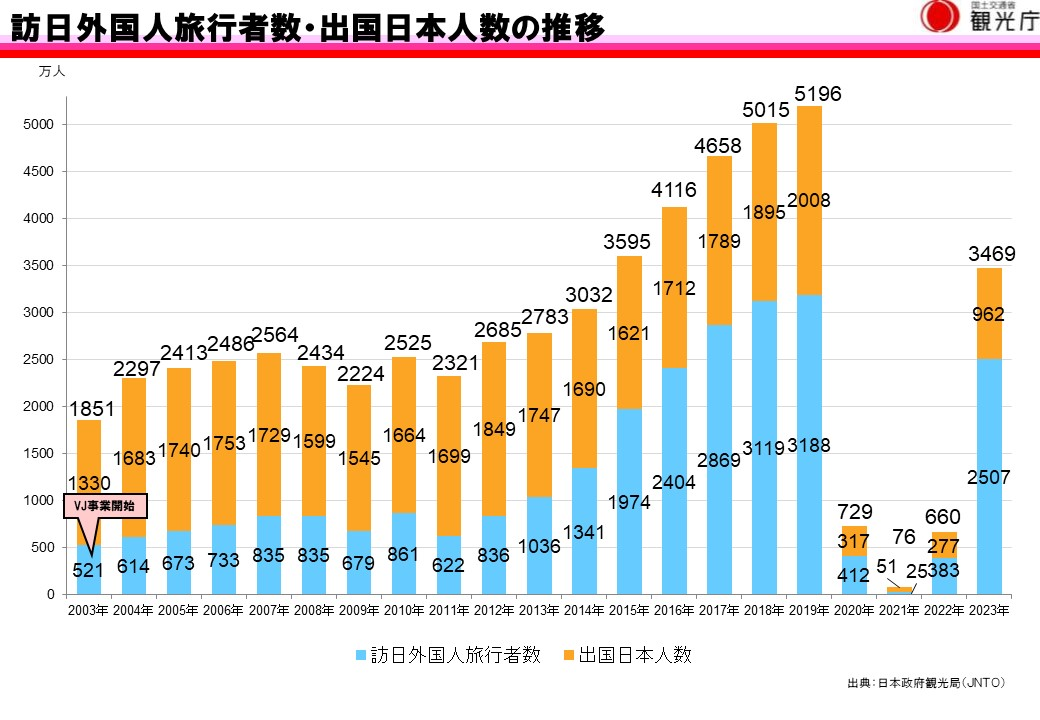
\includegraphics[width=0.8\textwidth]{Figures/001584918.jpg}
  \caption{2003年~2023年の訪日外国人旅行者数の推移} % TODO:いらないかも
  \label{fig:02} 
\end{figure}
上図を読み解くと,2003年から2019年にかけて,訪日外国人観光客数は倍以上に増加していることがうかがえる.2020年から2022年にかけては,著しく観光客数が減少しているが,これは新型コロナウイルスの世界的流行による影響であると考えられる.\par 
また,2023年は新型コロナウイルスによる行動自粛が解除されたことを受け,観光客数は2015年と同等水準まで回復しており,今後も増加するものと推察される.\par 
このような観光客数の急激な増加は,観光地の災害時の避難誘導タスクにおいて,以下のような問題を生じさせ適切な避難誘導を行えない可能性がある.
\begin{itemize}
  \item 観光客の土地勘がないため,的確な避難誘導が必要
  \item 観光客数は時間や季節によって変動するため,特定の避難所に多数の避難者が向かい,収容不足となる可能性がある.
  \item 避難誘導に従わずに周囲の人の動きに追従し,混乱を招く恐れがある.
\end{itemize}

\paragraph{観光地における避難誘導の課題}
ほとんどの観光客は土地勘がないとともに,防災意識もあまり高いとは言えない\cite{visitor01}.
ゆえに,単独では適切な避難行動がとれない可能性が高く,%TODO:地元住民との被害者数の比較について調査する..
このような,観光客の避難に関する問題は,多くの関連研究でも指摘されている.
%TODO:既存研究で指摘されている問題点をまとめる

\vspace{\baselineskip}
以上の背景から,今後発生しうる,南海トラフ地震などの巨大地震とそれにより発生する津波からの避難に関して,その対策は進められてきてはいるものの,地元住民だけでなく観光客も含めた避難に関しては多くの課題を残している現状がある.
また,避難する人だけでなく,避難者を適切な場所へ誘導する人員の安全確保にも課題が残されている.


\subsection{二次被害の発生}
津波避難誘導(あるいは,他の災害における避難誘導)においては,発災直後から二次被害にあう危険性が高い地域で活動しなければならないため,現場で誘導を行う警察や消防員等の安全確保が問題になっている.\par
\paragraph{風水害時における人的被害の特徴}
以下は,我が国で発生した1969年から2018年までの災害を対象に,消防団員が殉職した事例を消防白書や新聞記事,既往研究などから把握し,殉職時の状況を分析した結果が,山田らの研究\cite{yamada2020}によって報告されている.
\begin{quote}
  図-3 より,津波は,出動 途上,水防作業中,避難中,避難誘導中,人命救助中に 殉職者を出したことがわかった.なかでも避難誘導中と 避難中を合わせると全体で約 80\%を占めており,避難に関係する時に殉職者が出ている.
  \begin{figure}[H] 
    \centering 
    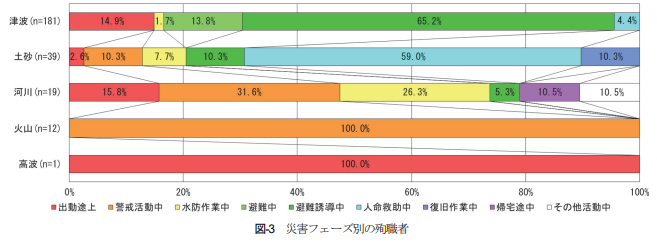
\includegraphics[width=0.8\textwidth]{Figures/fig-01.png}
    \caption{消防団員の災害フェーズ別殉職者の割合} 
    \label{fig:01} 
  \end{figure}
\end{quote}
以上より,津波災害時の消防団員おけるの2次被害に関しては,避難誘導中が最も多い結果であることが示されている.上記は消防団員に限定した統計であるが,同じく避難誘導を行うすべての人員においても同様の傾向があると推察される.\par
また,東日本大震災のケースにおいても,避難誘導にあたった警察職員や自治体職員の多数が地域住民の避難誘導中に津波に巻き込まれ殉職された事例\cite{touhoku-01}が報告されており,このような二次被害の防止は避難誘導において重要な意味を持つ.

\section{既存のドローンの災害対応における活用事例と航空法改正}
総務省・消防庁が公開しているデータ\cite{soumusho-01}によると、全国の消防本部におけるドローンの活用率は年々上昇しており、2017年には9.6\%だったものが,2021年には52.9\%と全国半数以上の消防本部でドローンの利活用が進めらたことが報告されている。
\begin{figure}[H] 
  \centering 
  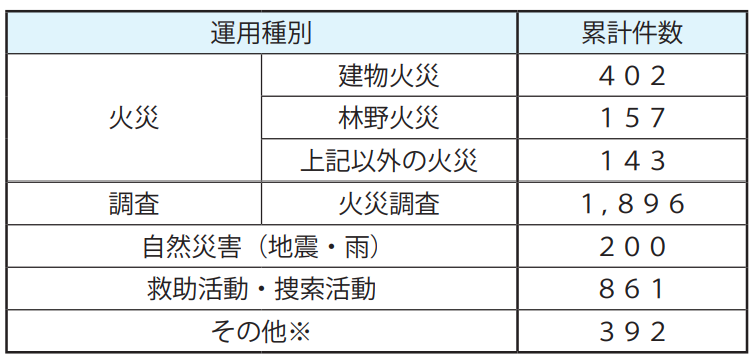
\includegraphics[width=0.6\textwidth]{Figures/2024-11-28 215911.png}
  \caption{ドローンの運用種別ごとの累計活用件数} 
  \label{fig:01} 
\end{figure}

加えて、我が国では,2022年に航空法が改正され,これまで規制されていたドローンの有人地帯目視外飛行(レベル4飛行\footnote{無人機の運用・操縦方法をレベル別に定めたもの.レベル4では操縦者が直接目視で機体を見ていなくても有人地帯でドローンを飛ばすことが可能になった.})が解禁された.
これにより,これまでドローンの活用が規制されていた防災分野での利活用や研究が大きく進んだ背景がある.\par 
\subsection{ドローンによる避難誘導の先行研究}



\section{強化学習}
%% TODO;機械学習と強化学習の基本的な枠組みについて述べる
  \subsection{MA-POCA(MultiAgent POsthumous Credit Assignment)}
  %% TODO: 協調学習:MA-POCAについての説明
\section{ナビゲーションメッシュ}
  \subsection{a* アルゴリズム}

